In this section, we examine the goodness of fit of the CAR model from several perspectives.
The autocorrelation function (ACF) and partial autocorrelation (PACF) are employed to examine the residuals from a temporal point of view.
Spatially, we display the residuals on the map and check for signs of systematic misprediction in any certain areas.  \\

To examine the residuals from a temporal perspective, the residuals are grouped based on their watershed membership, and averaged over all locations within the watershed.
The CAR model was initially fitted without autoregressive terms, and the ACF and PACF of residuals are given in Figure~\ref{fig:ACF_and_PACF}.
The  slow decay in the ACF plot and the cut-off pattern in the PACF plot suggest an addition of an AR(1) term in the CAR model.\\

\begin{figure}[htbp]
\begin{center}
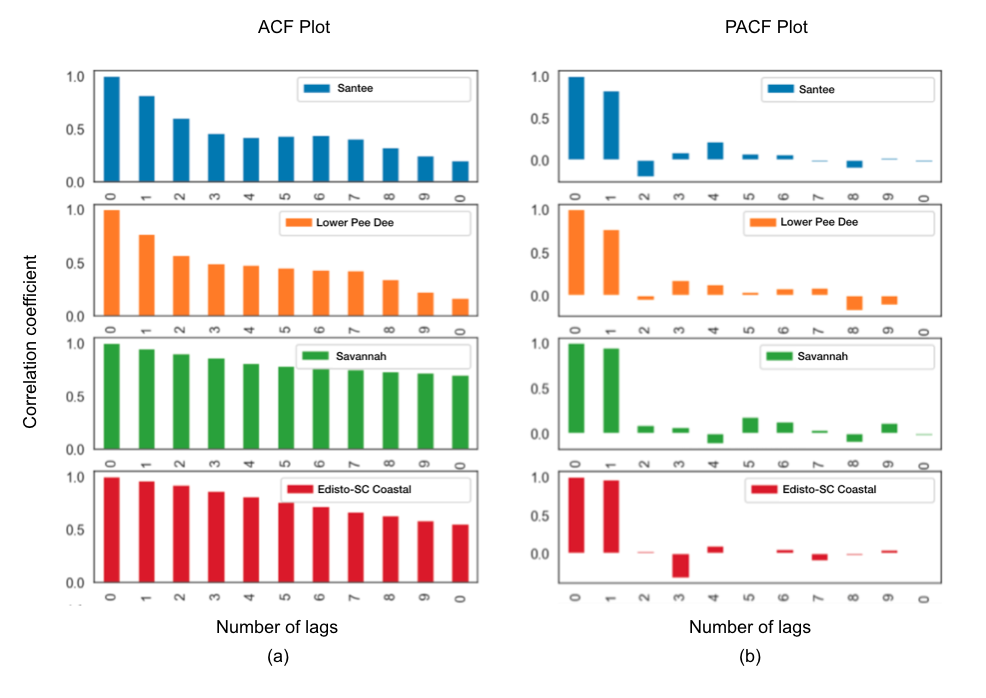
\includegraphics[width=0.8\textwidth]{../images/acf_and_pacf_for_residuals.png}
\caption{\hl{The ACF and PACF of residuals from the CAR model without autoregressive term.}}
\label{fig:ACF_and_PACF}
\end{center}
\end{figure}

To further evaluate the effectiveness of the autoregressive model, we show a time series plot (Figure~\ref{fig:resid_time_series}, left panel) after averaging out residuals spatially.
We also calculate the 2.5\% and 97.5\% percentiles, and thus the shaded area indicates the range of 95\% of all residuals.
 No apparent autocorrelation pattern is detected, although the last few  observations indicate increased volatility in  gage height.
 The absence of an autocorrelation pattern is attributed to the autoregressive term, since a  CAR model without the AR(1) term gives the residual time series plot that shows a more obvious autocorrelation  pattern and more variability (Figure~\ref{fig:resid_time_series}, right panel).\\

\begin{figure}[htbp]
\centering
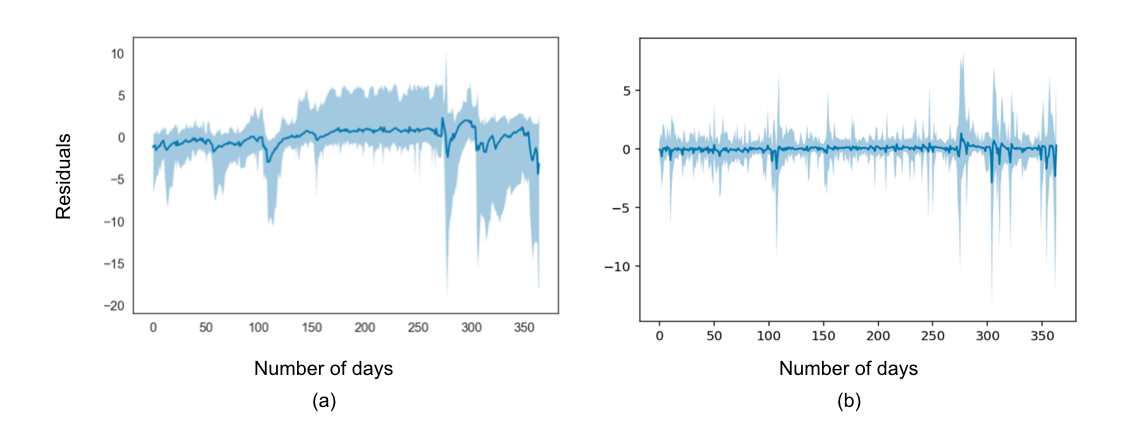
\includegraphics[width=1\textwidth]{../images/residuals_over_time_for_ar_and_non_ar.png}
\caption{\hl{The time series plot of residuals from the CAR model. The shaded area contains {95\%} of residuals at each time point. Left panel: with AR(1) term. Right panel: without AR(1) term.}}
\label{fig:resid_time_series}
\end{figure}

\hl{In addition, we examine several time series plots at multiple locations in Figure~{\ref{fig:per_site}}.
We picked four stations of varying degrees of volatility for demonstration purpose, each from a different HUC-6 area.
Station 02172002, for example, has rarely seen drastic changes in gage height over the five year between 2012
and 2016.
The only exception is during the 2015 flood event.
In contrast, Station 02197500 demonstrates a different pattern which is more variable and not dominated by the 2015
event.
Overall, the autoregressive model consistently captures the trend across different HUC-6 area locations
with no systematic overestimation or underestimation.
The calculation of mean squared error per site also validates this conclusion.} \\

\begin{figure}[htbp]
\centering
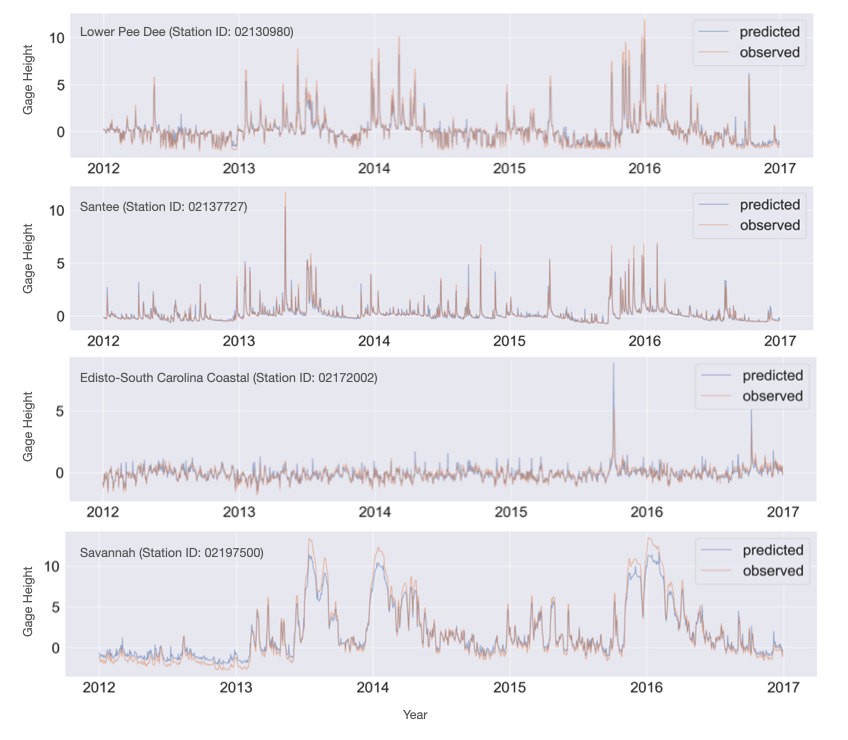
\includegraphics[width=1\textwidth]{../images/prediction_of_four_sites.png}
\caption{\hl{Time series plot of predicted gage height and observed gage height at multiple locations.}}
\label{fig:per_site}
\end{figure}

From a spatial perspective, we examine the distribution of residuals by visualizing them on a map with different colors representing \hl{negative and positive errors} (Figure~\ref{fig:spatial_resid}).
The radius of the circle is proportional to the residual.
This is a daily snapshot on October 3, 2015, from which one can conclude that the residuals are fairly evenly distributed.
Several randomly selected snapshots have been examined during the five-year span and no significant sign of overestimation or underestimation is observed.
 Additionally, one can  aggregate the residuals over a time period, for instance, a year, and make a yearly residual map for inspection.
 Such visualization presents a similar picture as Figure~\ref{fig:spatial_resid} and is thus omitted for the sake of space. \\

\begin{figure}
 \begin{center}
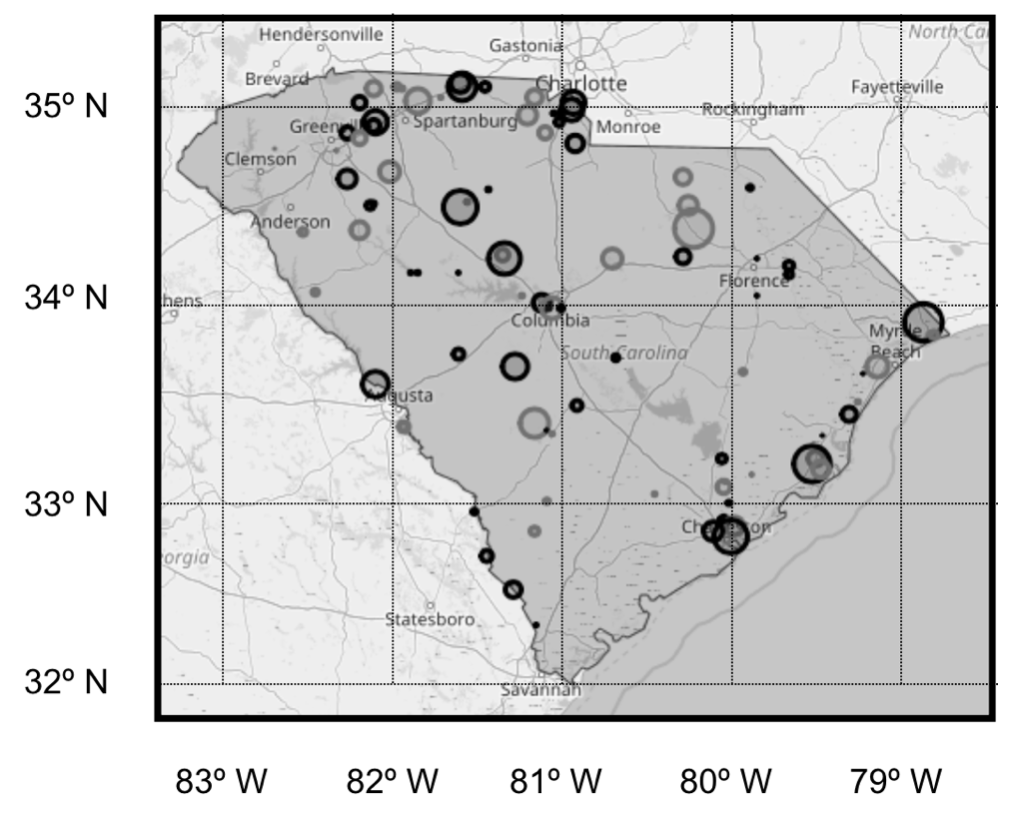
\includegraphics[width=0.6\textwidth]{../images/residuals_on_map.png}
\caption{The residuals from the CAR model on the map of SC. Gray circles indicate negative errors (overestimation) and black circles indicate positive errors (underestimation).}
\label{fig:spatial_resid}
 \end{center}
\end{figure}

Recall that our fitted model presented in Section~\ref{sec:model_fitting} used a non-normal error structure;
We now explain that choice.
If we fit a model with a normal error distribution and \hl{examine the qq (quantile-quantile) plot (Figure}~\ref{fig:hist_original}(b)), we perceive  a pattern that suggests heavy-tailed errors and thus a violation of normality.
This is potentially due to the heavy-tailed distribution of maximum gage heights \hl{(Figure}~\ref{fig:hist_original}(a)).
Note that the observations are plotted after the aforementioned scaling operation.
The data are also slightly skewed to the right possibly due to occasional thunderstorms, which cause short-term, sharp and severe rises in the gage heights.
\hl{Flow dynamics in the eastern US are mainly governed by landfall of tropical cyclones and extratropical systems.
Tail asymmetry can be partly related to the mixed dynamics forcing floods in different seasons (Smith, 2011)}.
Instead of normal errors, using an error structure that follows either a t or Laplace distribution handles extreme rainfall values better.
Specifically, we pick a t distribution with 3 degrees of freedom since $ \nu =3$ defines a distribution with reasonably heavy tails and  guarantees that both expectation and variance exist.
Alternatively, one can also set $\nu$ as a hyper-parameter which can be sampled from the posterior distribution.
\hl{Another possible error distribution could be a skew-t distribution, although for this data set the symmetric heavy-tailed error distributions provide a good fit}. \\

\begin{figure}[htbp]
 \begin{center}
     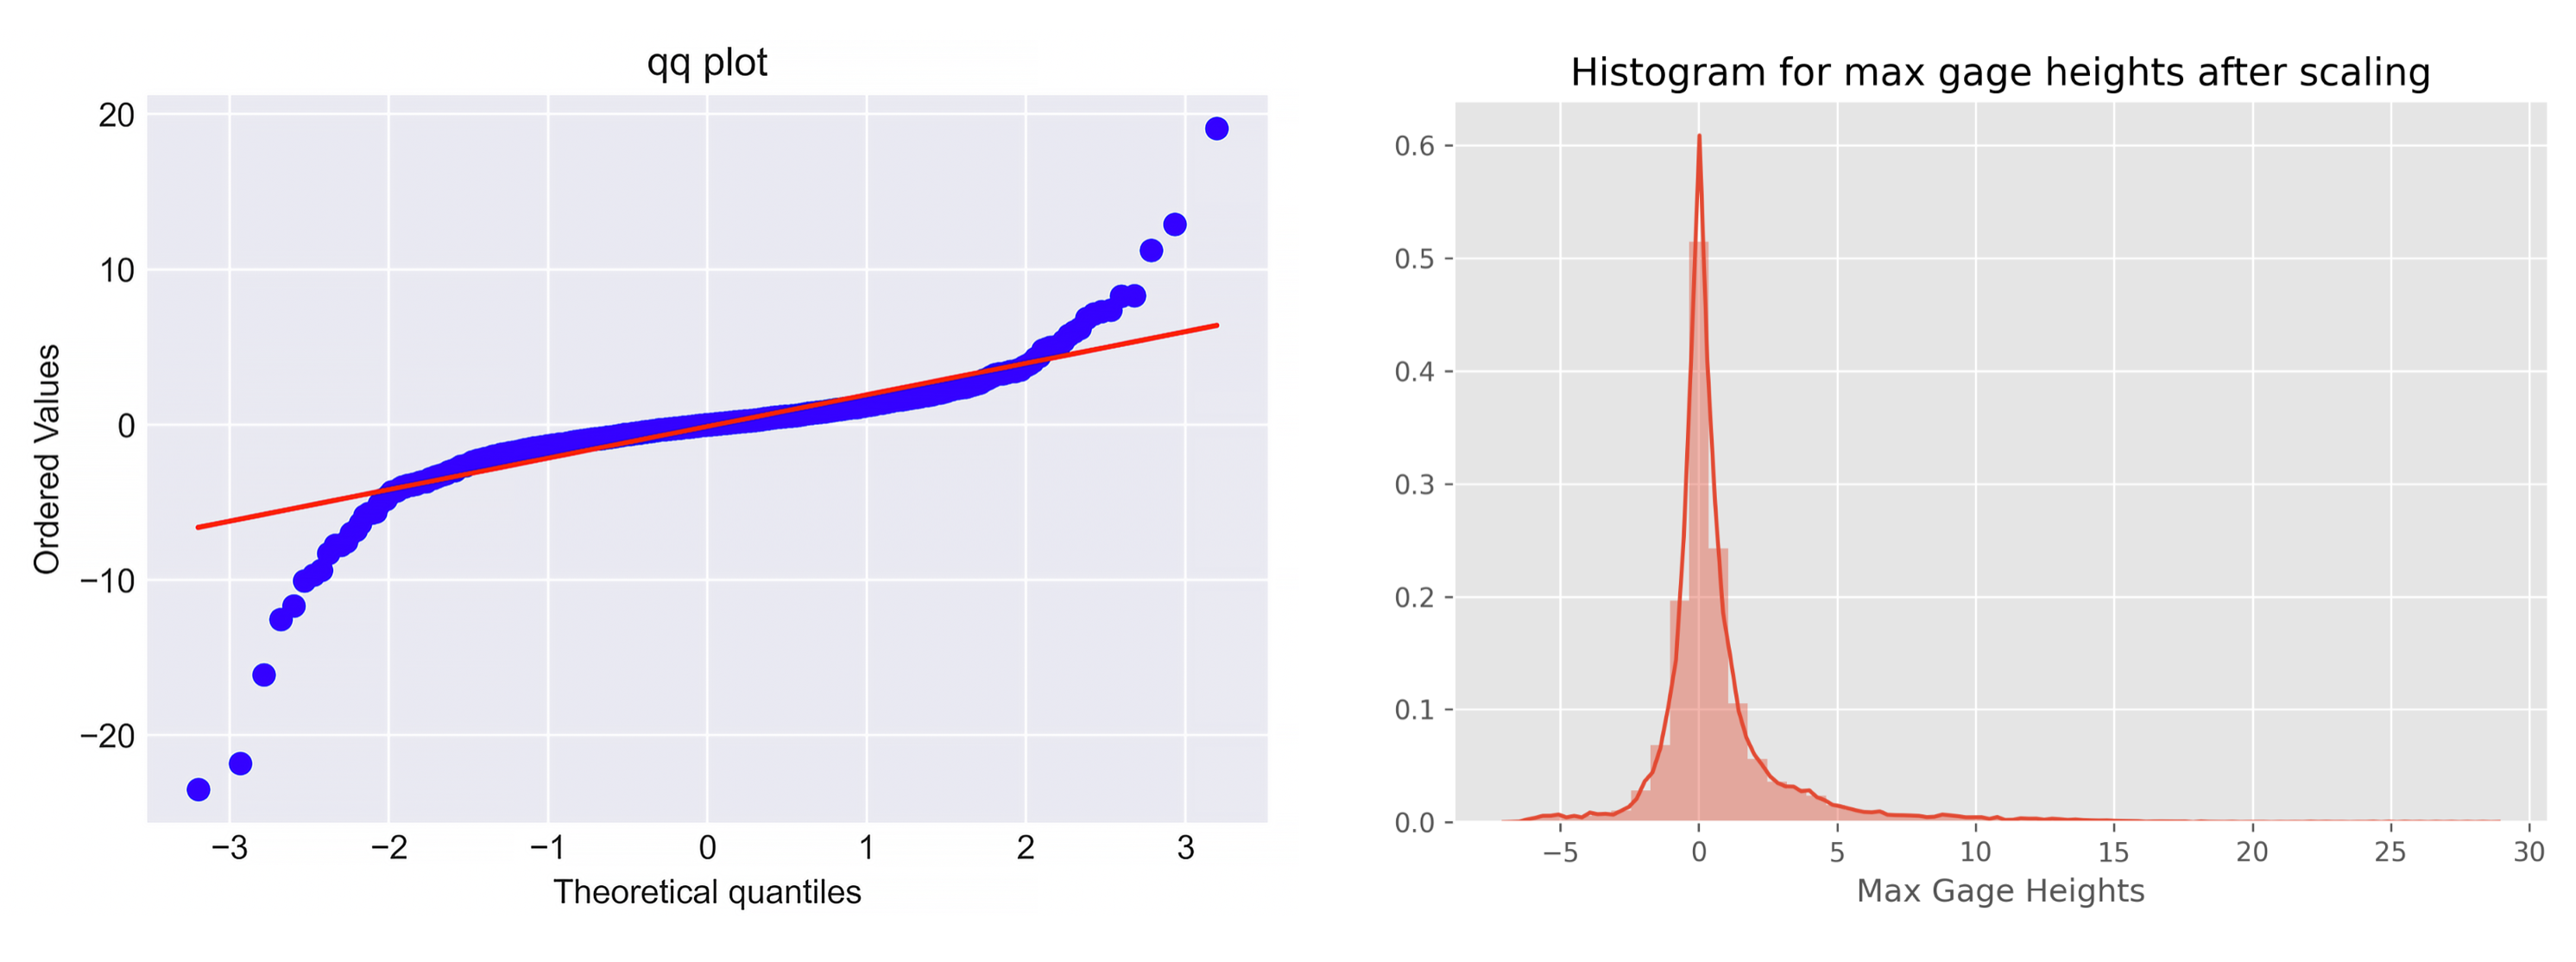
\includegraphics[width=\textwidth]{../images/qq_and_hist_gage_height_after_scaling.png}
\caption{(a): The histogram of gage heights after scaling. (b): The qq plot residuals assuming normal errors.}
\label{fig:hist_original}
 \end{center}
\end{figure}

The t distribution where $ \nu =3 $ (right panel, Figure~\ref{fig:qq_comp}) is slightly better in terms of its qq plot than the Laplace (left panel, Figure~\ref{fig:qq_comp}).
Hence, the estimation reported in section~\ref{subsec:reported_result} was based on the model assuming that the error term follows a t distribution with 3 degrees of freedom.
Note that the parameter estimates would be similar for the two models assuming either of the heavy-tailed distributions (t or Laplace).

\begin{figure}[htbp]
 \begin{center}
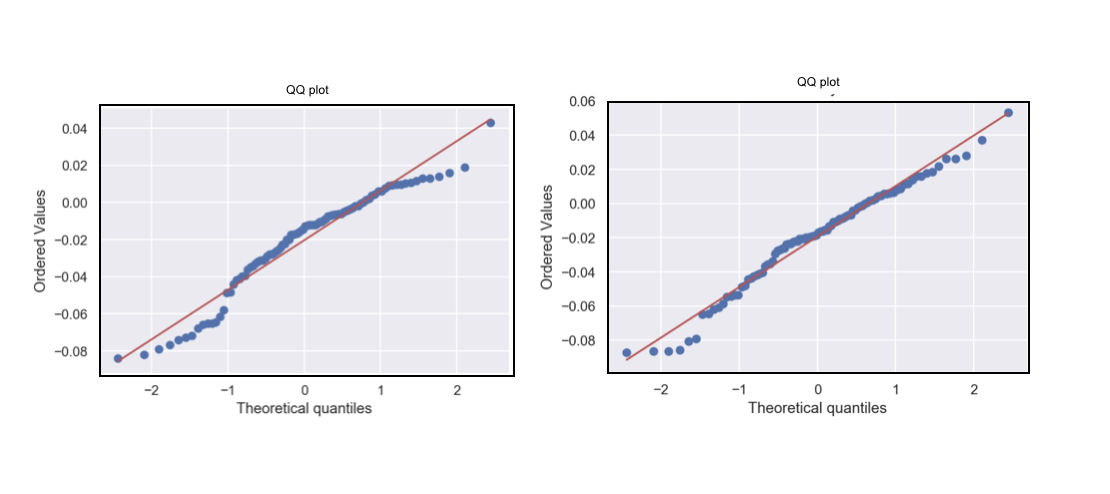
\includegraphics[width=1\textwidth]{../images/qq_plot_for_residuals.png}
\caption{The qq plots of residuals assuming Laplace (left) and t with 3 degrees of freedom (right) distributions.}
\label{fig:qq_comp}
 \end{center}
\end{figure}
